\documentclass{classrep}
\usepackage[utf8]{inputenc}
\usepackage{hyperref}
\usepackage{float}
\usepackage{graphicx}
\graphicspath{ {./} }
\usepackage{color}

\studycycle{Informatyka, studia dzienne, I st.}
\coursesemester{VI}

\coursename{Komputerowe systemy rozpoznawania}
\courseyear{2018/2019}

\courseteacher{dr inż. Marcin Kacprowicz}
\coursegroup{Wtorek, 16:15}

\author{
  \studentinfo{Paweł Młynarczyk}{210278} \and
  \studentinfo{Mateusz Kuźniarek}{210245}
}

\title{Zadanie 1 - Ekstrakcja cech, miary podobieństwa, klasyfikacja.}

\begin{document}
\maketitle

\section{Cel}
Celem zadania było zaprojektowanie i implementacja narzędzia, pozwalającego na klasyfikację tekstów przy użyciu algorytmu KNN. Podczas realizacji ćwiczenia, należało zbadać wpływ parametrów takich, jak sposób ekstrakcji cech, czy użyta miara podobieństwa na skuteczność i szybkość procesu klasyfikacji.

\section{Wprowadzenie}
\subsection{Ekstrakcja cech}
W celu szybkiego i efektywnego porównywania tekstów przydatna okazuje się ich reprezentacja w postaci wektora liczb. Współrzędne takiego wektora odpowiadają poszczególnym cechom, opisującym reprezentowany tekst. Proces analizy tekstu i określenia wartości liczbowej dla danej jego własności nazywamy ekstrakcją cech. Wybór odpowiedniego sposobu ekstrakcji jest kluczowy dla efektywnego działania programu. Niektóre ze sposobów opierają się na liście słów kluczowych.

Słowa te zostały wyznaczone przy pomocy przefiltrowanej listy słów, spośród której wybrano te wyrazy, które pojawiały się najczęściej.

\subsubsection{Wektor cech}
Używany do klasyfikacji wektor składał się z następujących cech:
\begin{itemize}
	\item Wartość TF dla każdego ze słów kluczowych.
	\item Wartośc podobieństwa każdego ze słóww kluczowych do analizowanego tekstu przy użyciu miary trigramów.
	\item Wartośc podobieństwa każdego ze słóww kluczowych do analizowanego tekstu przy użyciu uogólnionej miary n-gramów.
	\item Długość tekstu
	\item Średnia z występujących w tekście liczb
	\item Średnia długość słowa wśród 4 najdłuższych słów
\end{itemize}

\subsubsection{TF (Term Frequency)  \cite{TF_TF-IDF}}
Dla każdego słowa kluczowego obliczana jest jego częstotliwość przy pomocy wzoru: 
\begin{equation}
tf(t,d) =  \frac{f_{t,d}}{|d|} 
\end{equation}
gdzie \(f_{t,d}\) jest liczbą wsytąpień słowa \(t\) w tekście \(d\), a \(|d|\) jest liczbą wszystkich słów w tym tekście. Wartości funkcji \(tf(t,d)\) dla każdego słowa kluczowego stanową współrzędne wektora cech, reprezentującego dany dokument.

\iffalse
\subsubsection{TF-IDF (term frequency–inverse document frequency) \cite{TF_TF-IDF}} 
Ten sposób ekstrakcji cech wykorzystuje TF(Term Frequency) i wzbogaca je o informację na temat tego, jak często dane słowo znajduje się w dokementach innych niż analizowany. Wartość TF-IDF można uzyskać przy pomocy wzoru: 
\begin{equation}
tfidf(t,d,D) = tf(t,d) \cdot idf(t,D) 
\end{equation}
gdzie \(tf(t,d)\), jest wartością TF obliczoną przy pomocy woru 1., a \(idf(t,D)\) wyraża się wzorem
\begin{equation}
idf(t,D) = log\frac{|D|}{n} 
\end{equation}
gdzie \(|D|\) to liczba wszystkich tekstów w analizowanym zbiorze, a \(n\) to liczba tekstów, w których przynajmniej raz znajduje się słowo \(t\).
\fi

\subsection{Miara trigramów \cite{ANiewSkrypt}} 
Wartość podobieństwa tekstów przy użyciu miary trigramów obliczyć można z następującego wzoru:
\begin{equation}
sim_{n}(s_{1}, s_{2}) = \frac{1}{N-2}\sum_{i=1}^{N-2}h(i)
\end{equation}
 gdzie \(h(i) = 1\) jeśli 3-elementowy podciąg zaczynający się od i-tej pozycji występuje przynajmniej raz. W przeciwnym wypadku \(h(i) = 0\)
 
 \subsection{Uogólniona miara n-gramów \cite{ANiewSkrypt}} 
 Uogólniona miara n-gramów, w odróżnieniu od zwykłej miary n-gramów opiera się na podciągach różnych długości. Można ją obliczyć w następujący sposób.
 \begin{equation}
 sim_{n}(s_{1}, s_{2}) = \frac{2}{N^2+N}\sum_{i=1}^{N(s_1)}\sum_{j=j}^{N(s_1)-i+1} h(i,j)
 \end{equation}
 gdzie \(h(i,j) = 1\) jeśli i-elementowy podciąg zaczynający się od j-tej pozycji występuje przynajmniej raz. W przeciwnym wypadku \(h(i) = 0\)

\subsection{Normalizacja \cite{MLWiki}}
Otrzymane na powyższe sposoby cechy zostały następnie znormalizowane przy użyciu wzoru:
\begin{equation}
x' = \frac{x-x_{min}}{x_{max}-x_{min}} 
\end{equation}

\subsection{Algorytm KNN}
Do klasyfikacji tekstów wykorzystany został algorytm KNN(k-nearest neighbors). Pozwala on na przypisanie danej próbce klasy na podstawie tego, jak zaklasyfikowani są jej najbliżsi sąsiedzi. Bliskość dwóch próbek zdefiniowana jest za pomocą odpowiedniej metryki lub miary podobieństwa. \cite{KNNWiki}

W ramach zadania zaimplementowano następujące metryki: \newline
Metryka euklidesowa \cite{ANiewSkrypt}:
\begin{equation}
d(p,q) = \sqrt{\sum_{i=1}^{n} (p_{i} -q_{i})^{2}} 
\end{equation}
Metryka uliczna \cite{ANiewSkrypt}:
\begin{equation}
d(p,q) = \sum_{i=1}^{n} |p_{i} -q_{i}| 
\end{equation}
Metryka Czebyszewa \cite{ChebyshevWiki}:
\begin{equation}
d(p,q) = max_{i}(p_{i} -q_{i}) 
\end{equation}
gdzie \(n\) jest długością wektorów, \(p = [p_{1}, p_{2}, ..., p_{n}]\) oraz \(q = [q_{1}, q_{2}, ..., q_{n}]\) są wektorami, między którymi liczona jest odległość. 

Oprócz tego zaimplementowano następujące miary podobieństwa: \newline
Minimum-maximum \cite{ANiewSkrypt}
\begin{equation}
r_{mm}(p,q) = \frac{\sum_{i=1}^{n}min(p_{i},q_{i})}{\sum_{i=1}^{n}max(p_{i},q_{i})} 
\end{equation}
Średnia arytmetyczna-minimum \cite{ANiewSkrypt}
\begin{equation}
r_{am}(p,q) = \frac{\sum_{i=1}^{n}min(p_{i},q_{i})}{\frac{1}{2}\sum_{i=1}^{n}(p_{i}+q_{i})} 
\end{equation}
Własna propozycja miary podobieństwa
\begin{equation}
r_{wm}(p,q) = (r_{mm}(p,q))^{2}
\end{equation}

Powyższych metryk oraz miar podobieństw użyto do znalezieniu k najbliższych analizowanemu tekstowi próbek. Na ich podstawie tekst mógł zostać zaklasyfikowany do najbardziej licznej wśród wybranych sąsiadów z klas. W przypadku wielu jednakowo-licznych klas, wybierano tę, której próbka znajdowała się najbliżej analizowanego wektora.

\section{Opis implementacji}

W celu realizacji zadania została napisana aplikacja okienkowa w języku Java, natomiast graficzny interfejs użytkownika został wykonany w technologii JavaFX.
W projekcie skorzystano z natępujących bibliotek:
\begin{itemize}
	\item commons-io - bibliteka umożliwiająca deserializację plików xml; \cite{commons-io}
	\item javafx-fxml - biblioteka używana w warstwię prezentacji do reprezentacji graficznego interfejsu użytkownika; \cite{JavaFX}
	\item snowball-stemmer - biblioteka udostępniająca stemmer; \cite{Stemmer}
\end{itemize}

Projekt podzielono na dwa główne pakiety, przechowujący klasy warstwy prezentacji pakiet \textit{gui}, oraz pakiet \textit{logic}, w którym jest zawarta cała logika aplikacji. Na pakiet \textit{logic} składają się liczne podpakiety, które wydzielają poszczególne funkcjonalności aplikacji jeszcze bardziej. Są to: pakiet \textit{classification}, którego klasy realizują zagadnienie klasyfikacji obiektów tekstowych; pakiet \textit{extractors}, który zawiera w sobie ekstraktory cech; pakiet \textit{features} zawierający w sobie klasy, reprezentujące cechy obiektów; pakiet \textit{metrics}, którego klasy realizują poszczególne metryki; oraz pakiet \textit{utils} zawierający w sobie wszystkie klasy wspomagające działanie programu, niezwiązane bezpośrednio z ideą działania algorytmu knn. Podnadto w projekcie znajdują się pliki Scene.fxml oraz Styles.css, które opisują elementy graficznego interfejsu użytkownika.

Opis poszczególnych klas w ramach pakietu:

\begin{itemize}
	\item gui
	\begin{itemize}
		\item MainApp.java - klasa uruchomieniowa aplikacji, jej celem jest jedynie skonfigurowanie oraz ustawienie nowej sceny JavaFX;
		\item FXMLController.java - klasa kontrolera JavaFX przypisana do pliku FXML definiująca sposób działania elementów interfejsu użytkownika;
	\end{itemize}
	\item logic.classification
	\begin{itemize}
		\item TextSample.java - klasa reprezentująca próbkę tekstu, będąca reprezentacją badanych artykułów, zawiera informacje o etykiecie, i słowach zawartych w artykule;
		\item ExtractedSample.java - klasa reprezentująca wyekstrahowaną próbkę tekstu, na którą składa się jedynie etykieta oraz wektor cech tej próbki;
		\item Normalizer.java - klasa zdolna normalizować cechy wyekstrahowanej próbki do przedziału [0,1], w oparciu o cechy zbioru obiektów(tu zbioru treningowego);
		\item KNNClasification.java - reprezentacja algorytmu knn, do najważniejszych metod tej klasy należą metoda \textit{train()}, która bazując na zbiorze treningowym, tworzy odpowiednią strukturę, oraz metoda \textit{classify()} dokonująca klasyfikacji obiektów zbioru testowego w oparciu o utworzoną wcześniej strukturę;
	\end{itemize}
	\item logic.extraction
	\begin{itemize}
		\item FeatureExtractor.java - klasa abstrakcyjna reprezentująca wektor cech;
		\iffalse
		\item TFExtractor.java - klasa ekstraktora cechy TF;
		\item TFIDFExtractor.java - klasa ekstraktora cech TF-IDF;
		\fi
		\item CustomExtractor.java - klasa opracowanego na potrzeby zadania wektora cech;
	\end{itemize}
	\item logic.features
	\begin{itemize}
		\item Feature.java - klasa abstrakcyjna cechy;
		\item TermFrequency.java - klasa cechy TF;
		\iffalse
		\item TermFrequencyInverseDocumentFrequency.java - klasa cechy TF-IDF; 
		\fi
		\item CombinedTermFrequency.java - klasa cechy będącej sumą cech TF dla każdego słowa kluczowego z podanej listy.
		\item NGram.java - klasa cechy Ngramów;
		\item CombinedNGram.java - klasa cechy będącej sumą cech Ngramów dla każdego słowa kluczowego z podanej listy;
		\item Length.java - klasa cechy długości tekstu;
		\item AverageNumber.java - klasa cechy średniej arytmetycznej z liczb występujących w tekście;
		\item LongestWordsAverageLength.java - klasa cechy średniej arytmetycznej długości kilku najdłuższych słów występujących w tekście;
	\end{itemize}
	\item logic.metrics
	\begin{itemize}
		\item Metric.java - klasa abstrakcyjna metryki;
		\item EuclideanMetric.java - klasa reprezentacja metrykę Euklidesowską;
		\item ManhattanMetric.java - klasa reprezentacja metrykę Manhattańską (taksówkarską);
		\item ChebyshevMetric.java - klasa reprezentacja metrykę Czebyszewa;
		\item Similarity.java - klasa abstrakcyjna miary podobieństwa;
		\item MinMaxSimilarity.java - klasa reprezentacja miarę podobieństwa Minimum-Maximum;
		\item AverageMinSimilarity.java - klasa reprezentacja miarę podobieństwa Średniej Arytmetycznej-Minimum;
		\item CustomSimilarity.java - klasa reprezentująca własną miarę podobieństwa;
	\end{itemize}
	\item logic.utils
	\begin{itemize}
		\item SgmToXmlConverter.java - klasa konwertera zamieniająca plik sgm, w którym zostały dostarczone dane na plik, xml z którego są potem wczytywane do programu;
		\item ExampleLoader.java - klasa wczytująca teksty z pliku xml i przeprowadzająca wstępną obróbkę tekstu oraz stemizację, celem usprawnienia późniejszego procesu klasyfikacji;
		\item CSVData.java - klasa reprezentująca dane statystyczne zapisywane później do pliku csv;
		\item CSVWriter.java - klasa zapisująca dane powstałe w wyniku klasyfikacji do pliku csv;
	\end{itemize}
\end{itemize}

\begin{center}
	\begin{figure}[H]
		\advance\leftskip-3.65cm
		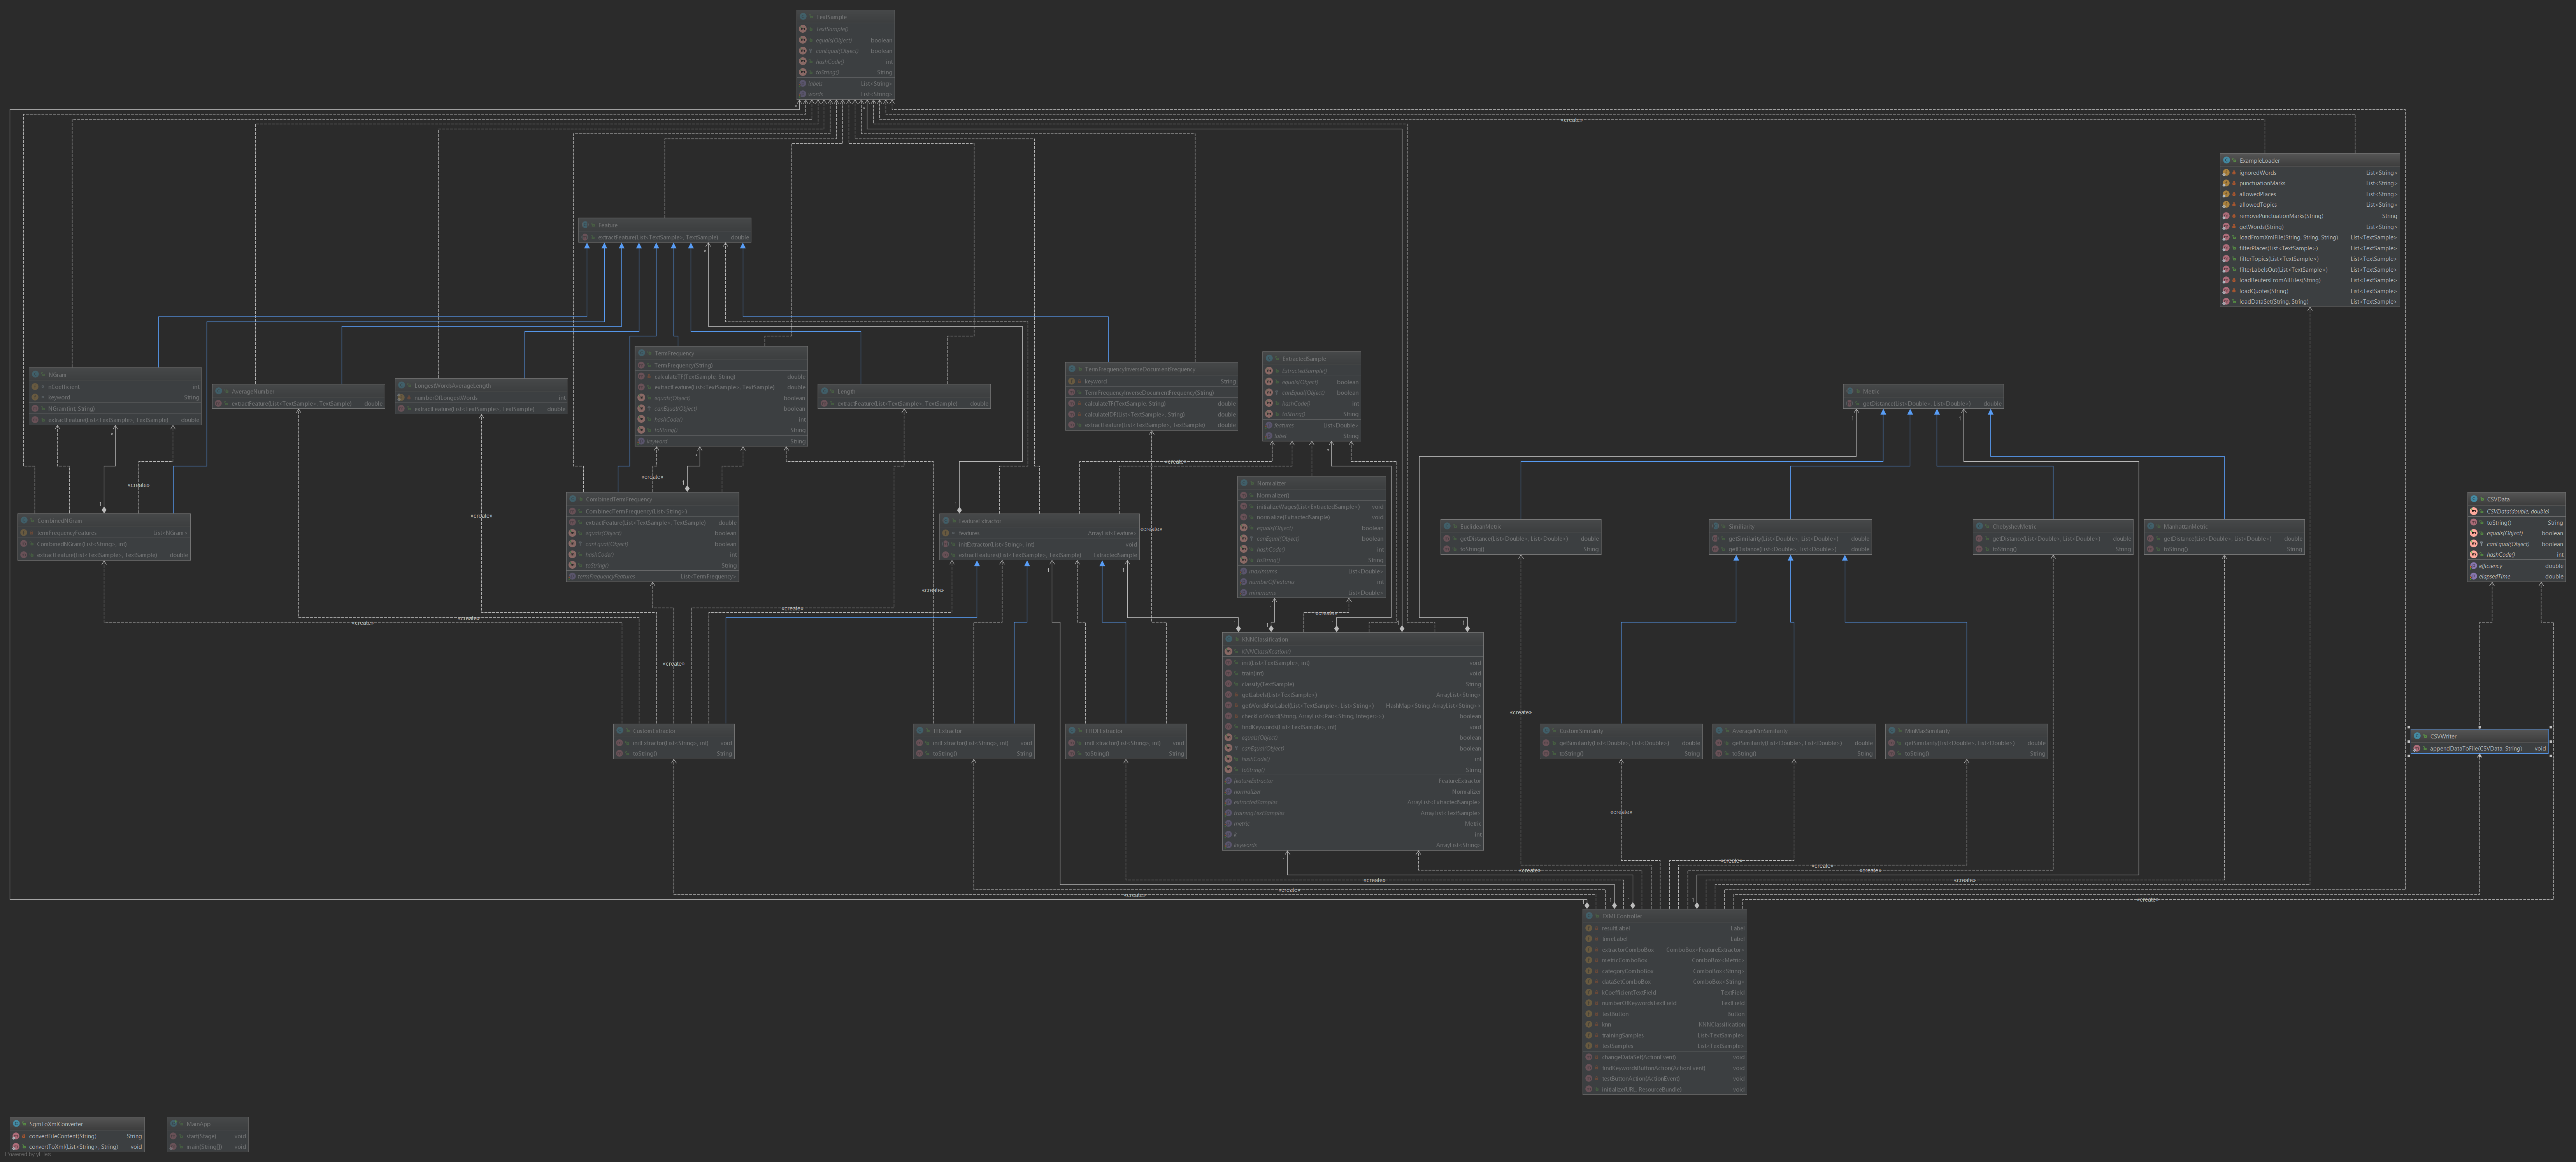
\includegraphics[width=\paperwidth]{ksr_uml}
	\end{figure}
\end{center}


\section{Materiały i metody}
Przed rozpoczęciem klasyfikacji analizowane teksty zostały odpowiednio przygotowane do wykorzystania. Treść została podzielona na pojedyncze słowa, które następnie zostały poddane procesowi stemmingu, który to polega na pozbyciu się końcówek fleksyjnych wyrazu. Z tekstu usunięto wszystkie znaki interpunkcyjne, a wielkie litery zamieniono na małe. Następnie, przy pomocy odpowiednio przygotowanej stop-listy, pozbyto się niepożądanych słów, które nie niosły ze sobą większego znaczenia dla procesu klasyfikacji.
Do eksperymentów użyto dwóch zbiorów danych. Własnoręcznie opracowany spis cytatów znanych pisarzy oraz dostępny pod \href{http://archive.ics.uci.edu/ml/datasets/Reuters-21578+Text+Categorization+Collection}{tym adresem} zbiór artykułów opublikowanych przez agencję prasową Reuters w 1987 r. W przypadku tego drugiego, dokonano klasyfikacji z uwagi na dwie kategorie.
\begin{itemize}
	\item places - Nazwa państwa, którego dotyczy artykuł. Podczas badań brano pod uwagę następujące wartości tej etykiety: west-germany, usa, france, uk, canada, japan.
	\item topics - Tematyka artykułu, przy badaniach wykorzystywano próbki o wartościach: earn, acq lub trade w tej kategorii.
\end{itemize}
W obu przypadakch pominięto artykuły, które nie zawierały informacji o danej kategorii lub klasyfikowały artykuł do dwóch lub więcej klas jednocześnie.

Podczas wszystkich eksperymentów odnotowywano skuteczność klasyfikacji (stosunek liczby poprawnie wytypowanych etykiet do liczby wszystkich próbek testowych) oraz czas klasyfikacji (w sekundach), na który składało się ekstrahowanie cech próbek ze zbioru treningowego jak i klasyfikacja próbek testowych. Każdy eksperyment został przeprowadzony 5 razy w celu wyliczenia średniego czasu wykonania.

Dostępne dane zostały podzielone na zbiór treningowy i testowy. Ten pierwszy stanowił bazę, na podstawie której algorytm klasyfikował podane mu próbki. Zbiór testowy został użyty do zbadania efektywności algorytmu w poniższych eksperymentach:
\subsection{Eksperyment 1. Wpływ wyboru sposobu ekstrakcji cech na klasyfikację}
Do zbadania wpływu sposobu ekstrakcji cech na klasyfikację wybrano metrykę euklidesową oraz wartośc parametru k równą 5. Następnie odnotowywano wyniki eksperymentu dla oryginalnego wektora cech, pomniejszonego o kolejne jego cechy, aby sprawdzić, jaki wpływ na proces klasyfikacji ma brak każdej z cech. Jako zbioru danych użyto artykułów agencji Reuters, a klasyfikacja odbywała się względem kategorii places. Liczba słów kluczowych wynosiła 3.
\subsection{Eksperyment 2. Wpływ parametru k na efektywność klasyfikacji}
Aby zbadać wpływ parametru k, przeprowadzono eksperyment przy użyciu metryki euklidesowej oraz 3 słów kluczowych. Następnie porównano wyniki dla odmiennych wartości parametru k. Eksperyment powtórzono dla różnych zbiorów danych i kategorii klasyfikacji. 
\subsection{Eksperyment 3. Wpływ wyboru metryki/miary podobieńśtwa na efektywność klasyfikacji}
Podczas tego eksperymentu wykorzystano zbiór artykułów agencji Reuters, 3 słowa kluczowe oraz parametr k o wartości 3. Klasyfikację przeprowadzono wględem kategorii places. Eksperyment powtórzono dla różnych metryk i miar podobieństwa.
\subsection{Eksperyment 4. Wpływ normalizacji na klasyfikację}
W tym eksperymencie użyto 3 słów kluczowych, metryki euklidesowej oraz współczynnika k równego 5. Badanie powtórzono w wariancie z normalizacją oraz bez niej dla różnych zbiorów danych i kategorii klasyfikacji.
\subsection{Eksperyment 5. Wpływ proporcji danych testowych i treningowych na klasyfikację}
W eksperymencie użyto metryki euklidesowej, 3 słów kluczowych oraz współczynnika k równego 5. Badanie powtórzono dla różnych proporcji danych testowych i treningowych. Eksperyment przeprowadzono dla różnych zbiorów danych i kategorii klasyfikacji.

\newpage
\section{Wyniki}
\subsection{Eksperyment 1. Wpływ wyboru ekstraktora cech na klasyfikację}
\begin{table}[H]
	\caption{Wpływ braku cechy w wektorze na proces klasyfikacji}
	\begin{tabular}{l|l|l}
		Cecha, o którą pomniejszony został wektor cech& skuteczność [\%]& czas wykonania [s]\\
		\hline
		Średnia liczba &78.191&140.316\\
		Długość tekstu &78.264&145.004\\
		Średnia długośc najdłuższych słów &78.191&150.325\\
		TF dla pierwszego słowa kluczowego &78.209&152.853\\
		Trigram dla pierwszego słowa kluczowego &78.209&135.604\\
		Uogólniony n-gram dla pierwszego słowa kluczowego &78.227&137.899\\
		TF dla drugiego słowa kluczowego &78.209&141.811\\
		Trigram dla drugiego słowa kluczowego &78.209&143.896\\
		Uogólniony n-gram dla drugiego słowa kluczowego &78.318&172.715\\
		TF dla trzeciego słowa kluczowego &78.209&138.575\\
		Trigram dla trzeciego słowa kluczowego &78.209&134.953\\
		Uogólniony n-gram dla trzeciego słowa kluczowego &78.209&126.521\\
	\end{tabular}
\end{table}

\subsection{Eksperyment 2. Wpływ parametru k na efektywność klasyfikacji} 
\begin{table}[H]
	\caption{Wpływ parametru k - zbiór danych Reuters}
	\begin{tabular}{l|l|l|l|l|l|l}
		Kategoria& \multicolumn{3}{|l}{ Reuters - places} 	& \multicolumn{3}{|l}{ Reuters - topics}\\
		\hline
		k& 3 & 7 & 9 & 3 & 7 & 9\\
		\hline
		skuteczność [\%]   &76.357&78.954&79.063&78.560&80.022& 80209\\
		czas wykonania [s] &74.521&78.675&73.751&14.706&13.890&14.326\\
	\end{tabular}
\end{table}
\begin{table}[H]
	\centering
	\caption{Wpływ parametru k - własny zbiór danych}
	\begin{tabular}{l|l|l|l}
		k& 3 & 7 & 9 \\
		\hline
		skuteczność [\%]   &47368&39473&36842\\
		czas wykonania [s] &0.001&0.002&0.001\\
	\end{tabular}
\end{table}

\subsection{Eksperyment 3. Wpływ wyboru metryki/miary podobieńśtwa na efektywność klasyfikacji}
\begin{table}[H]
	\centering
	\caption{Wpływ wyboru metryki/miary podobieńśtwa}
	\begin{tabular}{l|l|l}
		Metryka/Miara podobieństwa& skuteczność [\%] & czas wykonania [s]\\
		\hline
		Metryka euklidesowa&76.357&81.822\\
		Metryka taksówkarska&76.193&57.626\\
		Metryka Czebyszewa&76.302&25.019\\
		Średnia arytmetyczna-minimum&76.357&110.153\\
		Minimum-maximum&76.357&141.884\\
		Własna miara podobieńśtwa&76.357&148.490\\
	\end{tabular}
\end{table}

\subsection{Eksperyment 4. Wpływ normalizacji na klasyfikację}
\begin{table}[H]
	\caption{Wyniki z normalizacją}
	\begin{tabular}{l|l|l|l}
		Ekstraktor& Reuters - places & Reuters - topics & Własny zbiór danych\\
		\hline
		skuteczność [\%]   &78.209&79.985&47.368\\
		czas wykonania [s] &31.121&5.794&0.002\\
	\end{tabular}
\end{table}

\begin{table}[H]
	\caption{Wyniki bez normalizacji}
	\begin{tabular}{l|l|l|l}
		Ekstraktor& Reuters - places & Reuters - topics & Własny zbiór danych\\
		\hline
		skuteczność [\%]   &77.882&72.938&39.473\\
		czas wykonania [s] &17.353&2.851&0.001\\
	\end{tabular}
\end{table}

\subsection{Eksperyment 5. Wpływ proporcji danych testowych i treningowych na klasyfikację}
\begin{table}[H]
	\centering
	\caption{Wpływ proporcji danych testowych i treningowych na klasyfikację dla zbioru danych Reuters - kategoria topics}
	\begin{tabular}{l|l|l}
		Stosunek* & skuteczność [\%] & czas wykonania [s]\\
		\hline
		0.3&77.056&12.778\\
		0.5&71.175&17.088\\
		0.7&78.360&15.618\\
	\end{tabular}
\end{table}

\begin{table}[H]
	\centering
	\caption{Wpływ proporcji danych testowych i treningowych na klasyfikację dla zbioru danych Reuters - kategoria places}
	\begin{tabular}{l|l|l}
		Stosunek*& skuteczność [\%] & czas wykonania [s]\\
		\hline
		0.3&77.140&55.690\\
		0.5&77.626&81.213\\
		0.7&79.322&67.423\\
	\end{tabular}
\end{table}

\begin{table}[H]
	\centering
	\caption{Wpływ proporcji danych testowych i treningowych na klasyfikację dla własnego zbioru danych}
	\begin{tabular}{l|l|l}
		Stosunek*& skuteczność [\%] & czas wykonania [s]\\
		\hline
		0.3&45.454&0.004\\
		0.5&38.297&0.002\\
		0.7&44.827&0.002\\
	\end{tabular}
\end{table}

* Stosunek liczby danych treningowych do liczby wszystkich danych.
\newpage
\section{Dyskusja}
\subsection{Eksperyment 1. Wpływ wyboru ekstraktora cech na klasyfikację}
Bez względu na usuniętą cechę, czas wykonania klasyfikacji zmieniał się nieznacząco. Wynika to z faktu, że sam proces wyliczania wartości wektora cech jest niewielki w porównaniu do czasu, związanego z obliczaniem odległości między wektorami. Również skuteczność wahała się w niewielkim stopniu, co wynikać może z faktu, że w użytym w eksperymencie zbiorze danych agencji Reuters, znaczna większość artykułów posiada etykiete USA, co zmniejsza znaczenie dobranego wektora cech w procesie klasyfikacji.
\subsection{Eksperyment 2. Wpływ parametru k na efektywność klasyfikacji}
W tabeli 2. możemy zauważyć, że wraz ze wzrostem parametru k, skuteczność klasyfikacji zwiększyła się. Zupełnie inne wyniki widoczne są w tabeli 3. Dla zdefiniowanego na potrzeby zadania zbioru danych zwiększenie parametru k znacznie pogorszyło skuteczność. Wynika to z faktu, że dla większego k, mniej istotna jest odległość między próbkami, a na znaczeniu zyskuje ogólna liczba reprezentantów danej klasy w zbiorze danych. Efekt ten zaobserwowano we własnym zbiorze danych, ponieważ jest on mniej liczny. Zbyt mała wartość parametru k prowadzi do większego wpływu przypadkowych, odstających od reszty przedstawicieli swojej klasy, próbek. Zjawisko to można zaobserwować w tabeli 2. Liczba parametru k, powinna więc zostać odpowiednio dobrana, z uwagi na wielkość zbioru danych.
\subsection{Eksperyment 3. Wpływ wyboru metryki/miary podobieńśtwa na efektywność klasyfikacji}
Wśród sposobów na określanie bliskości pomiędzy wektorami możemy wyznaczyć dwie główne grupy - metryki oraz miary podobieństwa. Te pierwsze przyczyniły się do większej skuteczności klasyfikacji. Osiągnęły one także swój cel w krótszym czasie. Różnice pomiędzy skutecznością przedstawicieli tych samych grup jest niewielka. Wynikać to może z faktu, że przez sposób, w jaki zaimplementowane zostały miary podobieństwa, wymagają one dodatkowej operacji przeskalowania ich wartości na zbiór typowy dla metryk. Szczególnie efektywna okazała się metryka Czebyszewa, która osiągnęła największą skuteczność i najkrótszy czas wykonania dla parametrów opisanych w eksperymencie 3. 
\subsection{Eksperyment 4. Wpływ normalizacji na klasyfikację}
Zgodnie z oczekiwaniami, dla wszystkich zbiorów danych, normalizacja wydłużyła czas wykonania. We wszystkich przypadkach, normalizacja danych, zwiększyła efektywność klasyfikacji. Szczególny poprawę zaobserwowano dla własnego zbioru danych oraz dla artykułów agencji Reuters w kategorii topics. Wynikać to może z faktu, że wartości poszczególnych cech w wektorze mogą być bardziej lub mniej zróżnicowane w zależności od zbioru danych.
\subsection{Eksperyment 5. Wpływ proporcji danych testowych i treningowych na klasyfikację}
Zgodnie z oczekiwaniami, dla wszystkich zbiorów danych, normalizacja wydłużyła czas wykonania. We wszystkich przypadkach, normalizacja danych, zwiększyła efektywność klasyfikacji. Szczególny poprawę zaobserwowano dla własnego zbioru danych oraz dla artykułów agencji Reuters w kategorii topics. Wynikać to może z faktu, że wartości poszczególnych cech w wektorze mogą być bardziej lub mniej zróżnicowane w zależności od zbioru danych.

\newpage
\section{Wnioski}
\begin{itemize}
	\item Normalizacja jest użytecznym narzędziem w przypadku cech o zróżnicowanych wartościach.
	\item Wartość parametru k powinna być dopasowana do rozmiaru zbioru danych.
	\iffalse
	\item TFIDF może okazać się przydatny w sytuacjach, gdy czas wykonania programu nie ma większego znaczenia, a dobrane słowa kluczowe słabo identyfikują określone klasy.
	\fi
	\item Proces stemmingu może znacznie ułatwić pracę z klasyfikacją tekstu
	\item Sposób obliczania odległości między wektorami należy dobrać zarówno z uwagi na rodzaj danych jak i na sposób implementacji algorytmu KNN.
	\item Skorzystanie z odpowiednio zdefiniowanej stop-listy pozwala na wykluczenie z analizy mało użytecznych informacji.
	\item Algorytm KNN jest użytecznym, a zarazem stosunkowo prostym algorytmem klasyfikacji.
\end{itemize}

\begin{thebibliography}{0}
\bibitem{TF_TF-IDF}
Bernardi R., \textit{Term Frequency and Inverted Document Frequency}

\bibitem{ANiewSkrypt}
Niewiadomski A., \textit{Materiały, przykłady i ćwiczenia do przedmiotu Komputerowe Systemy Rozpoznawania}, 21 września 2009 

\bibitem{MLWiki}
http://mlwiki.org/index.php/Feature\_Normalization

\bibitem{KNNWiki}
Altman N. S., \textit{An introduction to kernel and nearest-neighbor nonparametric regression}, 1992

\bibitem{ChebyshevWiki}
James M. Abello, Panos M. Pardalos, Mauricio G. C. Resende \textit{Handbook of Massive Data Sets. Springer}, 2002

\bibitem{commons-io}
https://commons.apache.org/proper/commons-io/javadocs/api-2.5/index.html

\bibitem{JavaFX} 
https://docs.oracle.com/javase/8/javafx/api/toc.htm

\bibitem{Stemmer}
https://www.nltk.org/\_modules/nltk/stem/snowball.html

\end{thebibliography}
\end{document}
